\chapter{感觉系统}\label{ch:b3:sensory-systems}

在漆黑的夜晚，人眼能探测到几个光子的闪光——
这是物理上允许被探测到的最微弱的光量。
耳朵能够感知的声音，可使鼓膜移动的距离小于一个氢原子的直径，
并能分辨出相差仅百分之零点二的两个音调。
狗能追踪每立方厘米仅含几个分子的气味踪迹，
鲨鱼则借助心跳产生的电场，在沙下找到比目鱼。
每种感觉都始于一个细胞，
它把一种能量转换为膜电位的变化，而
每种感觉终于神经中的脉冲；二者之间，
正是本章要讨论的问题：感受器如何将单个分子或光子放大，
使之成为神经元可以读取的信号；如何把跨越万亿倍的强度范围，
压缩为每秒几百个脉冲的发放速率；
机械波如何按频率加以分拣；
上万种气味如何仅凭四百种受体加以区分；
大脑只接收脉冲，它又如何判断这些脉冲
来自哪一种感觉。

\section{所有感觉的共同原理}

\begin{definition}[转导、编码与适应]\label{def:b3:sensory-systems:principles}
\index{感觉转导}\index{受体电位}\index{标记线路}\index{感受野}\index{适应!感觉}\index{侧向抑制}
一个\emph{感受细胞}含有一种\emph{\omterm{def:b3:bacteriology:hgt}{转导}}机制
——即蛋白质或级联反应——它能把刺激
（光子、分子、位移、热或电场）转换为膜电导的变化，
进而产生\emph{受体电位}，其幅度随刺激呈分级变化；
细胞本身，或与之形成突触的神经元，把它转换为
一串动作电位，其发放速率编码刺激强度。信号的
\emph{感觉模态}并不取决于脉冲（各神经中的脉冲完全相同），
而取决于其所经由的神经通路及其在脑中的终点，
即一条\emph{标记线路}。感觉神经元只对
其\emph{感受野}内的刺激作出反应——一小片皮肤、视野中的一个区域、
一段频带——相邻感受野借助
\emph{侧向抑制}而彼此锐化，每个神经元抑制其邻居，
从而使边缘与反差被夸大。
大多数感受器会发生\emph{适应}：对持续刺激的反应逐渐下降，
因此它们报告的是变化而非水平，其工作范围
会移动到当前背景水平附近。
\end{definition}

\begin{theorem}[韦伯、费希纳与史蒂文斯]\label{thm:b3:sensory-systems:weber}
\index{韦伯定律}\index{费希纳定律}\index{史蒂文斯幂律}
韦伯（1834 年）的结论是：可察觉的最小变化
$\Delta I$ 占其强度 $I$ 的固定比例：
$\Delta I/I = k$，其中 $k$ 对重量约为 $0.02$，
对亮度约为 $0.08$，对响度约为 $0.1$。若把每个恰可察觉的差别
计为一个感觉单位 $S$，则 $\mathrm{d}S = \mathrm{d}I/
(kI)$，并有
\[
S = \frac{1}{k}\ln\frac{I}{I_{0}} ,
\]
其中 $I_{0}$ 为阈值：感觉随刺激的对数增长，
这就是强度常以\omterm{def:b3:sensory-systems:cochlea}{分贝}和星等来度量的原因（费希纳，1860 年），
也解释了为何一支蜡烛加到另一支蜡烛上会被察觉，
而加到泛光灯上则不会被察觉。直接标度实验
让受试者为感觉赋予数值，结果则给出
幂律 $S \propto I^{n}$（史蒂文斯，1957 年），其中 $n \approx
0.3$ 对应响度和亮度，$1$ 对应线段长度，$3.5$ 对应
电击；在几个数量级的范围内，对数与小幂指数
几乎无法区分，二者在本质上一致：神经系统
对刺激进行了压缩。
\end{theorem}
\begin{proof}
由 $\Delta I = kI$（取 $S$ 的一个单位），感觉的增量
与刺激增量之比为 $\mathrm{d}S/\mathrm{d}I = 1/(kI)$；
从阈值 $I_{0}$（此时 $S = 0$）积分，得 $S = (1/k)
\ln(I/I_{0})$。幂律则基于另一假设：刺激的一个固定
\emph{比值}引起感觉的一个固定\emph{比值}，
$\mathrm{d}S/S = n\,\mathrm{d}I/I$，其积分为 $S \propto I^{n}$；
当 $n \to 0$ 并选取适当标度时，它趋于对数。
\end{proof}

\begin{omfigure}
\begin{tikzpicture}
\begin{axis}[
  width=0.68\linewidth, height=5.6cm,
  xmode=log,
  xmin=1, xmax=1e6, ymin=0, ymax=15,
  xlabel={刺激强度 $I/I_{0}$}, ylabel={感觉 $S$（任意单位）},
  xlabel style={font=\small, at={(axis description cs:0.5,-0.12)}, anchor=north}, ylabel style={font=\small},
  tick label style={font=\small}, ytick={0,5,10,15},
  clip=false,
]
\addplot[very thick, omDef, domain=1:1e6, samples=100] {ln(x)};
\addplot[very thick, omThm, domain=1:1e6, samples=100] {0.235*x^0.3 - 0.235};
\addplot[very thick, omMeth!70!black, domain=1:1e6, samples=100] {0.5*x^0.24 - 0.5};
\node[font=\scriptsize, omDef, anchor=north west] at (axis cs:2,10.2) {费希纳：$S = \ln(I/I_{0})$};
\node[font=\scriptsize, omThm, anchor=south east] at (axis cs:9e5,0.4) {史蒂文斯：$S \propto I^{0.3}$};
\node[font=\scriptsize, omMeth!70!black, anchor=north west] at (axis cs:2,12.5) {史蒂文斯：$S \propto I^{0.24}$};
\end{axis}
\end{tikzpicture}

{\small 将百万倍的强度范围压缩为
一种增长缓慢的感觉：费希纳的对数律与史蒂文斯的幂律
小指数的幂律在几个数量级内难以区分，二者
都说明感觉报告的是比值而非差值。}
\end{omfigure}

\section{视觉}

\begin{definition}[视网膜]\label{def:b3:sensory-systems:retina}
\index{视网膜}\index{视杆细胞}\index{视锥细胞}\index{光转导}\index{视紫红质}\index{神经节细胞}\index{中心–周边}
\emph{视网膜}是位于眼球后部的一层脑组织，由三层细胞构成，
其中光感受器反常地位于最后方，
紧贴色素上皮。\emph{视杆细胞}——每只眼 $10^{8}$ 个，只含一种色素，
即\emph{视紫红质}——负责弱光视觉，白天时饱和；
\emph{视锥细胞}——$6\times 10^{6}$ 个，三种色素的峰值分别位于蓝、
绿、红区，密集分布于中央凹——负责日间视觉、色觉和
视敏度。\emph{光\omterm{def:b3:bacteriology:hgt}{转导}}是一个级联反应：一个光子使一个视紫红质的
视黄醛发色团发生异构化；被激活的视紫红质启动
数百个 G~蛋白\omterm{def:b3:bacteriology:hgt}{转导}素分子，每个分子又
激活一种磷酸二酯酶，后者分解环 GMP；环 GMP 的下降
cGMP 减少使暗中由 cGMP 维持开放的阳离子通道关闭，
内向的“暗电流”停止，细胞发生\emph{超极化}——
光使光感受器关闭，释放的谷氨酸减少。在
暗处，细胞去极化并持续释放递质。信号
经\emph{双极细胞}传递（分 ON 型和 OFF 型两类，分别使信号
反转或保持），再传至\emph{\omterm{def:b3:nervous-systems:comparative}{神经节}细胞}，每只眼一百万个，
其轴突构成视神经——这里实现了一百倍的压缩。
水平细胞和无长突细胞横向联系，其抑制作用
使每个\omterm{def:b3:nervous-systems:comparative}{神经节}细胞具有\emph{中心–周边}\omterm{def:b3:sensory-systems:principles}{感受野}：
中央圆盘区域受光兴奋，环状周边区域受光抑制
（或相反），因此视网膜所报告的是局部对比
与边缘，而非绝对光照。
\end{definition}

\begin{omfigure}
\begin{tikzpicture}[every node/.style={font=\scriptsize}, >=stealth]
  % cascade boxes with amplification numbers
  \node[draw, thick, rounded corners, fill=omProp!30, align=center] (ph) at (0,0) {1 个光子};
  \node[draw, thick, rounded corners, fill=omDef!20, align=center] (rh) at (2.6,0) {1 个视紫红质*\\(metarhodopsin II)};
  \node[draw, thick, rounded corners, fill=omDef!20, align=center] (tr) at (5.6,0) {$\sim 500$ 个转导蛋白 \\被激活};
  \node[draw, thick, rounded corners, fill=omDef!20, align=center] (pde) at (8.6,0) {$\sim 500$ 个 PDE 被激活：\\$\sim 10^{5}$ 个 cGMP 被水解};
  \node[draw, thick, rounded corners, fill=omThm!20, align=center] (ch) at (5.6,-2.0) {$\sim 200$ 个阳离子通道关闭；\\暗电流下降 \qty{1}{pA}};
  \node[draw, thick, rounded corners, fill=omMeth!25, align=center] (out) at (1.4,-2.0) {超极化 \qty{1}{mV}；\\谷氨酸释放减少};
  \draw[->, thick] (ph) -- (rh); \draw[->, thick] (rh) -- (tr); \draw[->, thick] (tr) -- (pde);
  \draw[->, thick] (pde.south) |- (ch.east); \draw[->, thick] (ch) -- (out);
  \node[below, font=\tiny, align=center] at (7.1,-2.8) {每一步都使信号放大；整个级联在 \qty{200}{ms} 内由 \\视紫红质激酶、抑制蛋白和转导蛋白的 GTP 酶终止，随后复位};
\end{tikzpicture}

{\small \omterm{def:b3:sensory-systems:retina}{光转导}作为放大器。一个被吸收的光子经两级催化，关闭
数百个通道，分子数上的增益约为
一百万倍——足以使单个光子在\omterm{def:b3:sensory-systems:retina}{视杆细胞}中产生
可测电流。}
\end{omfigure}

\begin{theorem}[计数光子：看见的频率]\label{thm:b3:sensory-systems:hecht}
\index{单光子探测}\index{看见频率曲线}\index{泊松!光子计数}
一次闪光平均向一小片\omterm{def:b3:sensory-systems:retina}{视杆细胞}提供 $a$ 个被吸收的光子，
每次呈现时，所提供的光子数 $k$ 服从
泊松分布：$P(k) = e^{-a}a^{k}/k!$。若观察者在至少吸收 $n$ 个光子时
报告看见闪光，
则看见的概率为
\[
P_{\text{看见}}(a) = 1 - \sum_{k=0}^{n-1} e^{-a}\,\frac{a^{k}}{k!} ,
\]
该曲线由 $0$ 上升到 $1$，且随 $a$ 增大而升高，其
\emph{陡峭程度}在 $a$ 的对数标度上仅取决于 $n$：
阈值计数越大，曲线越陡。因此，拟合
实测的\omterm{thm:b3:sensory-systems:hecht}{看见频率曲线}即可得出 $n$，
而无需知道送达的光子中实际有多少被吸收。
\end{theorem}
\begin{proof}
来自弱而稳定光源的光子独立随机到达，并且
在平均为 $a$ 的短闪光中，被吸收的光子数服从泊松分布
（即二项分布在光子数很多、每个光子被吸收概率很小时的极限）。
看见要求 $k \ge n$，其概率为 1 减去
前 $n$ 项泊松项之和。将光源强度乘以因子 $c$，
则 $a$ 乘以 $c$，曲线沿 $\log a$ 轴平移，
形状不变，因此形状可以确定 $n$：当 $n =
1$ 时 $P = 1 - e^{-a}$ 在 $a$ 的两个数量级内上升；当 $n = 6$ 时
则在不到一个数量级内上升。
\end{proof}

\begin{proof}[证据]
赫克特、施莱尔和皮雷纳（1942）让观察者在黑暗中待了
半小时，然后在\omterm{def:b3:sensory-systems:retina}{视网膜}\omterm{def:b3:sensory-systems:retina}{视杆细胞}丰富的周边区域闪一个微小的绿色光点，
每次闪光持续一毫秒，共闪了数百次，光强分几档，
并记录被看见的闪光比例。阈值闪光
在角膜处约含 $90$ 个光子，其中（经反射和眼内介质吸收后，
再计入到达\omterm{def:b3:sensory-systems:retina}{视杆细胞}的光子被\omterm{def:b3:sensory-systems:retina}{视紫红质}吸收的概率 $20\,\%$）约
$5$--$14$ 个被吸收。
\omterm{thm:b3:sensory-systems:hecht}{看见频率曲线}的陡峭程度相当于
$n = 5$ 到 $7$：观察者回答“是”时，约有六个\omterm{def:b3:sensory-systems:retina}{视杆细胞}，
即光斑下五百个中的六个，各自捕获了一个光子。单个
\omterm{def:b3:sensory-systems:retina}{视杆细胞}只能探测一个光子，大脑则要求几个光子同时到达，
以免\omterm{def:b3:sensory-systems:retina}{视杆细胞}的自发异构化造成误报——
每个\omterm{def:b3:sensory-systems:retina}{视杆细胞}约每四十秒一次——低于恒星光子的速率。
\end{proof}

\begin{omfigure}
\begin{tikzpicture}
\begin{axis}[
  width=0.68\linewidth, height=5.6cm,
  xmode=log,
  xmin=0.1, xmax=100, ymin=0, ymax=1.05,
  xlabel={每次闪光平均吸收的光子数，$a$}, ylabel={看见的概率},
  xlabel style={font=\small, at={(axis description cs:0.5,-0.12)}, anchor=north}, ylabel style={font=\small},
  tick label style={font=\small}, ytick={0,0.5,1},
  clip=false,
]
\addplot[very thick, omDef, domain=0.1:100, samples=120] {1-exp(-x)};
\addplot[very thick, omProp, domain=0.1:100, samples=120] {1-exp(-x)*(1+x+x^2/2)};
\addplot[very thick, omThm, domain=0.1:100, samples=120] {1-exp(-x)*(1+x+x^2/2+x^3/6+x^4/24+x^5/120)};
\node[font=\scriptsize, omDef, anchor=north west] at (axis cs:0.12,0.95) {$n = 1$};
\node[font=\scriptsize, omProp, anchor=north west] at (axis cs:1.1,0.5) {$n = 3$};
\node[font=\scriptsize, omThm, anchor=north west] at (axis cs:5.5,0.45) {$n = 6$};
\end{axis}
\end{tikzpicture}

{\small 阈值为一、三和六个被吸收光子时的\omterm{thm:b3:sensory-systems:hecht}{看见频率曲线}。
曲线越陡，同时到达所需的光子数越多。赫克特的
观察者得到的曲线与红色曲线相似。}
\end{omfigure}

\begin{omfigure}
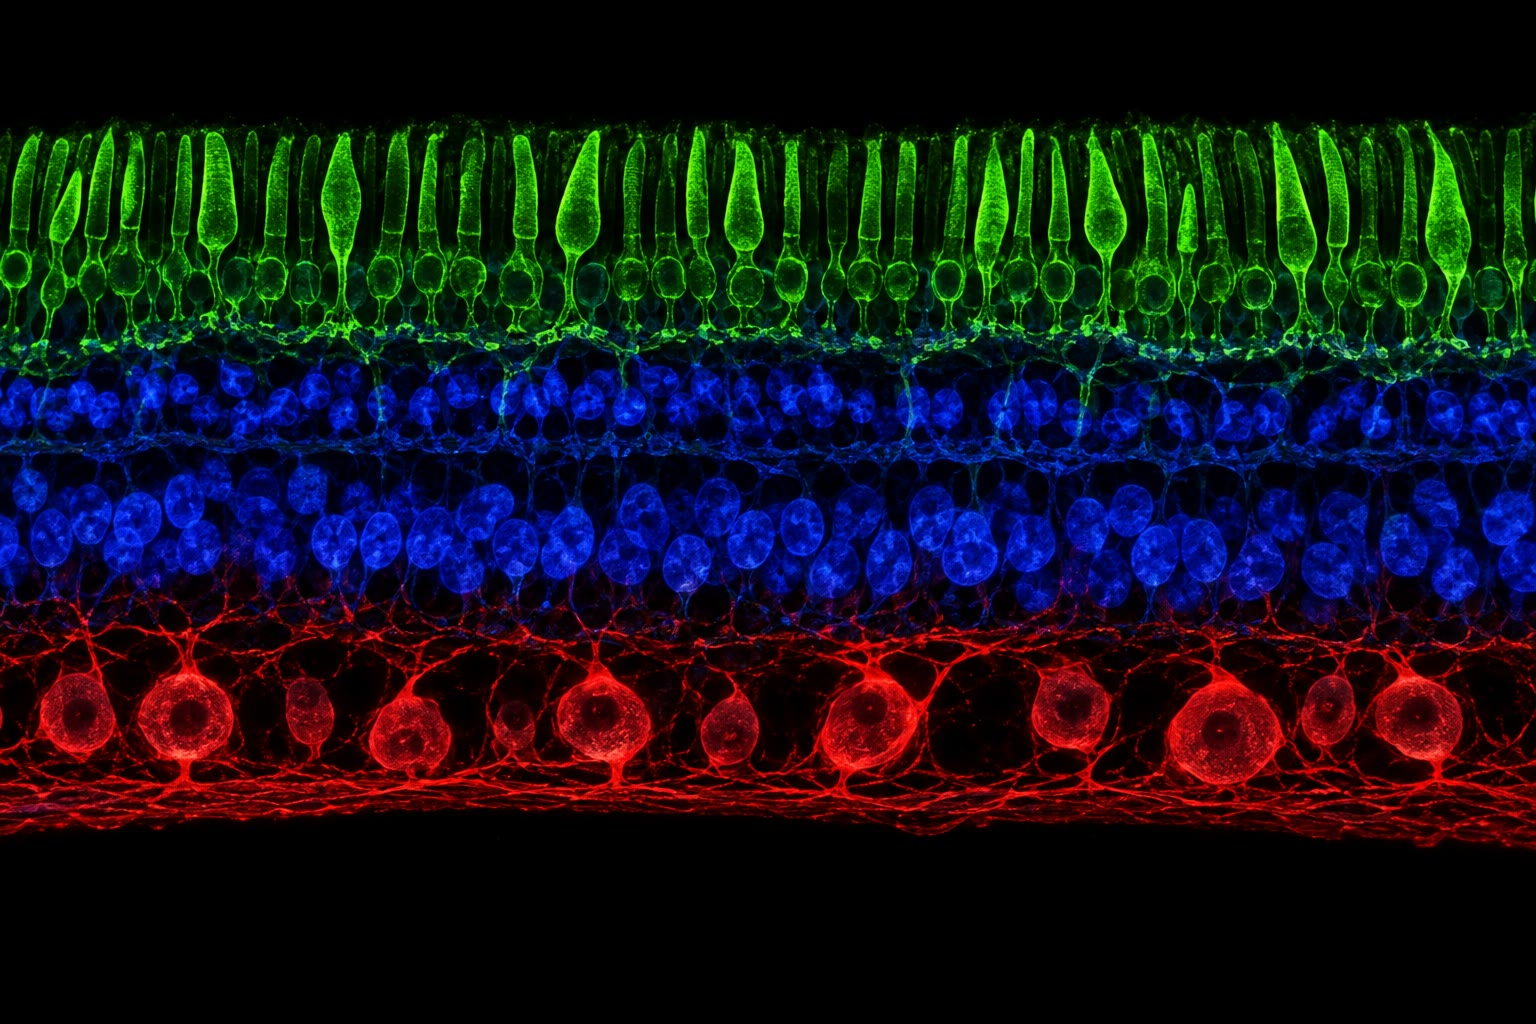
\includegraphics[width=0.46\linewidth]{images/book5/ai/b5-18-retina-section.jpg}\hspace{0.04\linewidth}
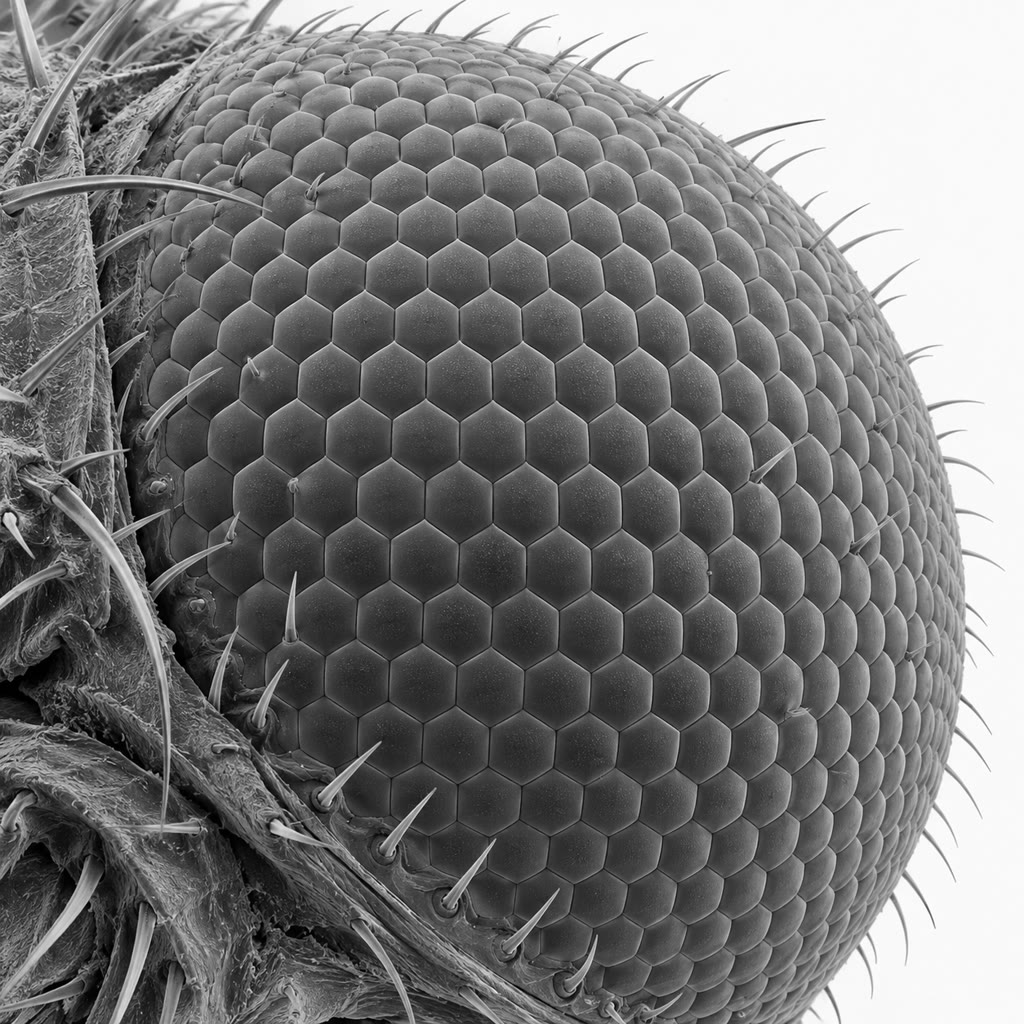
\includegraphics[width=0.36\linewidth]{images/book5/ai/b5-18-compound-eye.jpg}

{\small 左：\omterm{def:b3:sensory-systems:retina}{视网膜}切片，光感受器（绿色）位于
后部，依次是双极细胞和水平细胞，再是\omterm{def:b3:sensory-systems:retina}{神经节细胞}（红色），
其轴突通向大脑。右：苍蝇的复眼，
由数百个独立的透镜组成，每个透镜各配有自己的感受器——
解决同一问题的另一种方案。}
\end{omfigure}

\section{听觉与平衡}

\begin{definition}[耳蜗]\label{def:b3:sensory-systems:cochlea}
\index{耳蜗}\index{基底膜}\index{音调定位}\index{毛细胞}\index{静纤毛}\index{顶连接}\index{分贝}
声音是压力波；耳朵要解决的问题是探测
空气中仅几十微帕的压强变化，并按频率对其分类。
鼓膜和三块中耳听小骨将
鼓膜（\qty{55}{mm^2}）上的力集中到卵圆窗（\qty{3}{mm^2}）上，
使压强约提高二十倍——这正是空气与内耳液体间的
阻抗匹配，若无此匹配，大部分
声音将被反射。在\emph{耳蜗}内，一条盘绕的管道
全长 \qty{35}{mm}，压力波沿\emph{基底膜}传播，
该膜基部窄而硬，顶部宽而软；每个频率
使膜在某一处振动最强——高频在基部，
低频在顶部——形成\emph{音调定位}图谱，
大脑将其读作音调。膜上排布着
\emph{毛细胞}：单排共 \num{3500} 个内毛细胞，
每个细胞顶端冠以一束\emph{静\omterm{def:b3:cytoskeleton-motility:cilia}{纤毛}}，\omterm{def:b3:cytoskeleton-motility:cilia}{纤毛}尖端之间以
细小的\emph{顶连接}相连；\omterm{def:b3:cytoskeleton-motility:cilia}{纤毛}束向最高的\omterm{def:b3:cytoskeleton-motility:cilia}{纤毛}弯曲时，连接被拉紧，
并在微秒内拉开阳离子通道，无需第二信使，
钾离子从内淋巴流入，
内淋巴成分特殊，其 $+\qty{80}{mV}$ 的电位
给出 \qty{150}{mV} 的驱动力。内毛细胞向听神经发出信号；
而 \num{12000} 个外毛细胞受同样运动驱动，
随声音借助马达蛋白 prestin 收缩与伸长，
并将能量泵回膜的振动中——这是一个
放大器，使调谐锐化一百倍，多数耳聋正源于它的失灵。
强度以\emph{分贝}计量：$L = 10\log_{10}
(I/I_{0})$，其中 $I_{0} = \qty{1e-12}{W/m^2}$ 为听阈；
人耳的工作范围超过 \qty{120}{dB}，强度跨度达一万亿倍。
\end{definition}

\begin{omfigure}
\begin{tikzpicture}[every node/.style={font=\scriptsize}, >=stealth]
  % unrolled cochlea
  \begin{scope}
    \draw[thick, omDef, fill=omDef!10] (0,0.9) -- (7,1.4) -- (7,-1.4) -- (0,-0.9) -- cycle;
    \draw[very thick, omProp] (0,0.15) -- (7,-0.15); \draw[very thick, omProp] (0,-0.15) -- (7,0.15);
    \node[above] at (0.8,1.05) {基底：窄而硬}; \node[above] at (6.2,1.5) {顶端：宽而松软};
    \node[left, align=right] at (-0.1,0) {卵圆窗 \\（来自镫骨）};
    \foreach \x/\f in {0.9/\qty{16}{kHz}, 2.3/\qty{4}{kHz}, 3.8/\qty{1}{kHz}, 5.4/\qty{250}{Hz}, 6.6/\qty{60}{Hz}} { \draw[omThm, thick] (\x,-0.55) -- (\x,0.55); \node[below, omThm] at (\x,-0.65) {\f}; }
    \node[below, align=center] at (3.5,-1.7) {基底膜（橙色）：各频率在某一处振动最强 \\——音调定位};
  \end{scope}
  % hair cell mechanism
  \begin{scope}[xshift=8.2cm, yshift=-0.6cm]
    \draw[thick, fill=omMeth!20] (0,0) rectangle (1.6,1.2); \node[below] at (0.8,-0.05) {毛细胞};
    \foreach \x/\h in {0.35/0.6, 0.65/0.85, 0.95/1.1, 1.25/1.35} \draw[very thick, omMeth!70!black] (\x,1.2) -- (\x,1.2+\h);
    \foreach \x/\h/\xx/\hh in {0.35/0.6/0.65/0.85, 0.65/0.85/0.95/1.1, 0.95/1.1/1.25/1.35} \draw[omThm, thick] (\x,1.2+\h) -- (\xx,1.2+\hh-0.1);
    \draw[->, thick] (1.9,2.3) -- (2.4,2.3) node[right, align=left, font=\tiny] {向最高的一排弯曲：\\顶连接拉伸，通道 \\在 $\unit{\micro s}$ 内开放；K$^{+}$ 流入 \\（\qty{150}{mV} 驱动）};
    \node[above, align=center] at (0.8,2.7) {静纤毛由 \\顶连接相连（红色）};
  \end{scope}
\end{tikzpicture}

{\small 左：展开的\omterm{def:b3:sensory-systems:cochlea}{耳蜗}——\omterm{def:b3:sensory-systems:cochlea}{基底膜}由
硬到软逐渐过渡，各频率在各自位置达到峰值。右：一束
\omterm{def:b3:sensory-systems:cochlea}{毛细胞}\omterm{def:b3:cytoskeleton-motility:cilia}{纤毛}，其\omterm{def:b3:sensory-systems:cochlea}{顶连接}
在\omterm{def:b3:cytoskeleton-motility:cilia}{纤毛}束弯曲时机械地打开\omterm{def:b3:bacteriology:hgt}{转导}通道。}
\end{omfigure}

\begin{proof}[证据]
冯·贝凯西（1940 年代）解剖尸体的\omterm{def:b3:sensory-systems:cochlea}{耳蜗}，将
银粉撒在\omterm{def:b3:sensory-systems:cochlea}{基底膜}上，并在频闪光下观察，
纯音在\omterm{def:b3:sensory-systems:cochlea}{基底膜}上形成行波，音调越高，峰值
越靠近基底——即位置编码，他因此
于 1961 年获得诺贝尔奖。哈德斯佩思（1980 年代）用玻璃纤维推动
一束\omterm{def:b3:sensory-systems:cochlea}{毛细胞}\omterm{def:b3:cytoskeleton-motility:cilia}{纤毛}并记录电流：电流在推动后
\qty{10}{\micro s} 内即流动，远快于任何酶促级联，
其大小与\omterm{def:b3:cytoskeleton-motility:cilia}{纤毛}束向最高一排移动的距离成正比，
并在\omterm{def:b3:sensory-systems:cochlea}{顶连接}被钙螯合剂切断后消失。
门控是机械性的——连接牵拉使通道打开 ---
这正是听觉为各种感觉中最快的原因，也是其
\omterm{def:b3:bacteriology:hgt}{转导}器被使连接断裂的强声摧毁的原因。
\end{proof}

\begin{example}[耳的数值]\label{ex:b3:sensory-systems:ear-numbers}
在听阈处，\omterm{def:b3:sensory-systems:cochlea}{基底膜}约移动
\qty{0.1}{nm}，压强振幅为 \qty{20}{\micro Pa}，
约为大气压的十亿分之二；在 \qty{120}{dB} 时，压强
是其一百万倍，膜的运动达数十纳米。年轻人的
耳朵可听 \qty{20}{Hz} 至 \qty{20}{kHz} 的声音，并能分辨相隔
\qty{0.3}{\%} 的音调，位置编码的分辨力由
外\omterm{def:b3:sensory-systems:cochlea}{毛细胞}增强。听神经的 \num{30000} 条神经纤维
与压力波同步放电，直至约 \qty{4}{kHz}（锁相），
其携带的时间精度可达数十微秒，大脑由此
依据声音到达两耳的时间差计算声源方向，
时间差可小至 \qty{10}{\micro s}。平衡器官利用
同样的\omterm{def:b3:sensory-systems:cochlea}{毛细胞}：在\emph{半规管}中，液体的
惯性在头部转动（角加速度）时使其弯曲；在
耳石器官中，一层碳酸钙晶体使\omterm{def:b3:sensory-systems:cochlea}{毛细胞}承受
重力与线加速度的载荷。
\end{example}

\begin{omfigure}
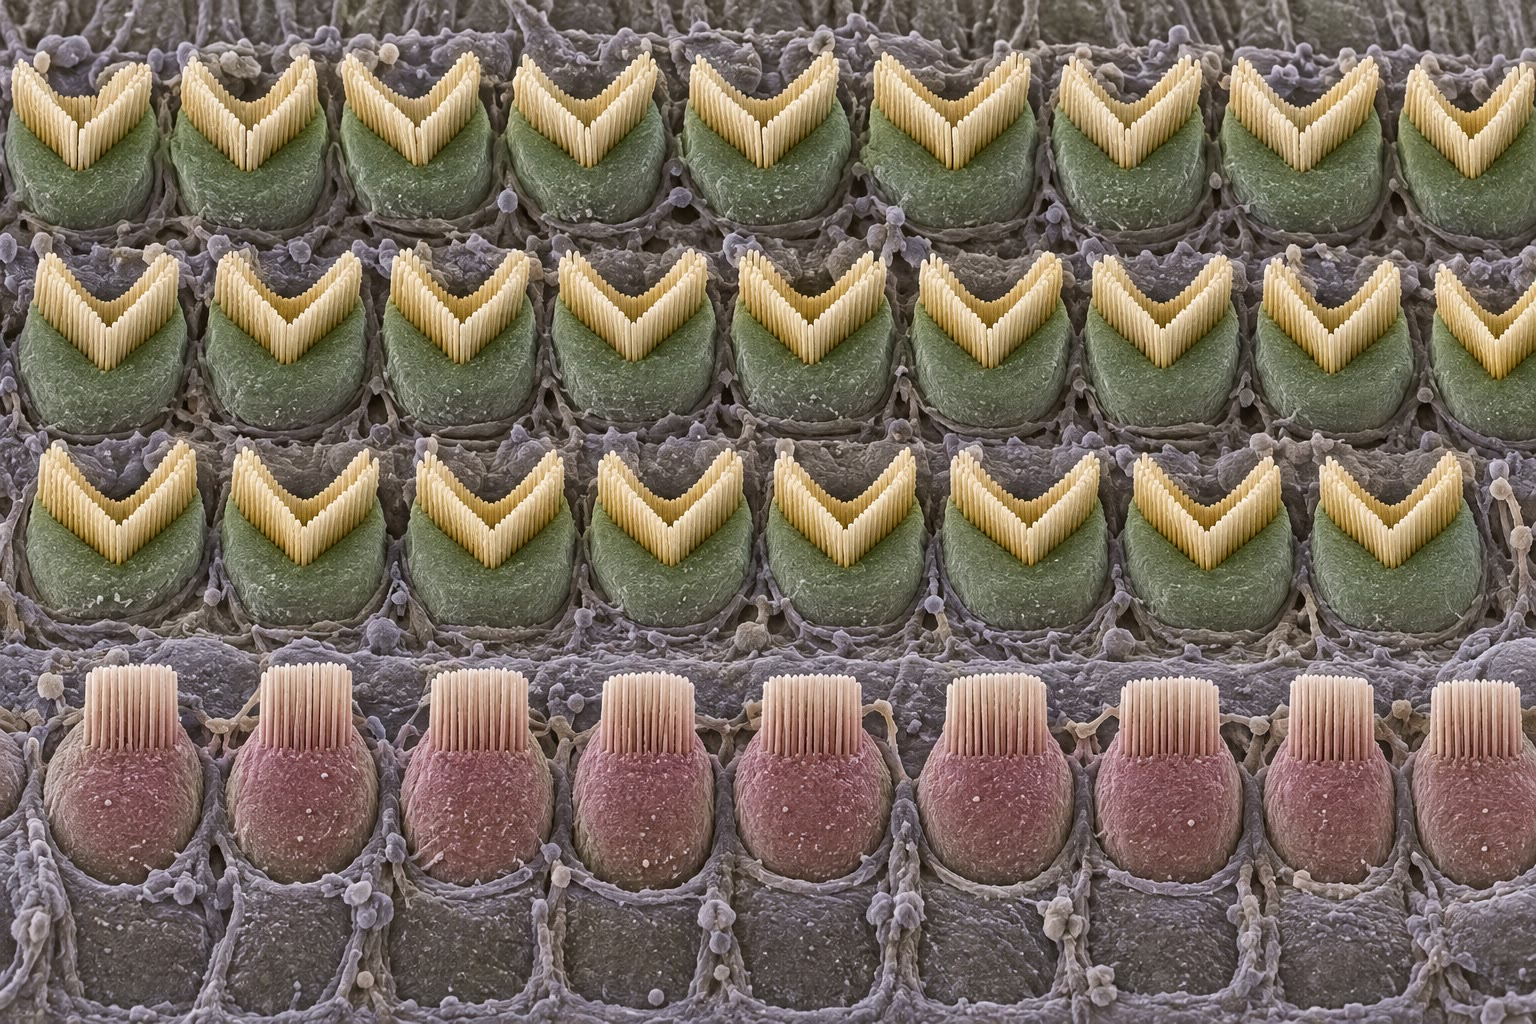
\includegraphics[width=0.54\linewidth]{images/book5/ai/b5-18-cochlea-hair-cells.jpg}

{\small 从上方看到的科蒂器官：三排外\omterm{def:b3:sensory-systems:cochlea}{毛细胞}
呈 V 形的\omterm{def:b3:cytoskeleton-motility:cilia}{纤毛}束，一排内\omterm{def:b3:sensory-systems:cochlea}{毛细胞}。每个\omterm{def:b3:cytoskeleton-motility:cilia}{纤毛}束的\omterm{def:b3:sensory-systems:cochlea}{顶
连接}打开通道；外\omterm{def:b3:sensory-systems:cochlea}{毛细胞}放大信号，内\omterm{def:b3:sensory-systems:cochlea}{毛细胞}
传递信号。}
\end{omfigure}

\section{化学感觉}

\begin{definition}[嗅觉与味觉]\label{def:b3:sensory-systems:chemical}
\index{嗅觉受体}\index{组合编码}\index{小球}\index{味觉}
嗅觉始于鼻腔顶部的一片上皮，其中
约 1000 万个\emph{嗅觉感觉神经元}各自表达
一个\emph{嗅觉受体}基因，人类中共约 $400$ 个（小鼠为 \num{1100} 个，
在两种基因组中均为最大的基因家族）——G 蛋白偶联
受体，在结合口袋中结合气味分子，并通过
环 AMP 打开通道。每种受体可结合多种气味分子，
每种气味分子也可结合多种受体，因此一种气味是
一种\emph{组合编码}，即 $400$ 种受体类型上的活动模式，
而分子中一个碳原子的改变即会改变
该模式及气味。表达同一种受体的全部神经元
将轴突投射到嗅球中同一个或两个\emph{小球}，
因此嗅球构成一张图谱，每种气味是一种空间
活跃小球模式，由皮层读取而不经过
\omterm{def:b3:nervous-systems:plan}{丘脑}。味觉较简单：五种感觉模态，每种都是
来自各自受体细胞的\omterm{def:b3:sensory-systems:principles}{标记线路}——甜味、鲜味和苦味，
通过 G 蛋白偶联受体（甜味受体一种，鲜味受体一种，
约二十五种苦味受体），咸味通过钠通道，酸味通过
质子通道——而我们所说的风味其余部分则是
嗅觉，经口腔后部到达鼻腔。
\end{definition}

\begin{proof}[证据]
巴克与阿克塞尔（1991）推断，气味受体应为
仅在嗅上皮中表达的 G 蛋白偶联受体，
并用简并\omterm{def:b3:genetic-engineering:pcr}{引物}通过 PCR 找到一个由数百个
此类基因组成的家族，它们仅在该处表达——即
一个世纪以来未知的\omterm{def:b3:sensory-systems:chemical}{嗅觉受体}。原位杂交显示，
每个神经元表达一种受体，同类神经元\omterm{def:b3:nervous-systems:circuits}{汇聚}于单个\omterm{def:b3:sensory-systems:chemical}{小球}。
马尔尼克、巴克及同事（1999）记录了单个神经元，发现
每种气味分子可激活多种受体，每种受体
也可被多种气味分子激活——即\omterm{def:b3:sensory-systems:chemical}{组合编码}。布什迪德及同事
（2014）让受试者辨别混合气味，估计
人类能区分的气味超过一万亿种，远超
人们通常认为的数千种。
\end{proof}

\begin{proposition}[组合编码的容量]\label{prop:b3:sensory-systems:combinatorial}
\index{组合编码!容量}
设 $R$ 种受体各自处于活跃或沉默状态，则一种气味可由
$2^{R}$ 种模式之一表示；取 $R = 400$ 时，此数为
$10^{120}$；即使只考虑恰有 $10$ 种受体活跃的模式，
其数目仍有 $\binom{400}{10} \approx 3\times 10^{20}$。
分辨能力受限，并非由编码本身，而是由受体的噪声
与大脑的解读所限。若采用每种气味一个受体的\omterm{def:b3:sensory-systems:principles}{标记线路}编码，
只能区分 $400$ 种气味，而\omterm{def:b3:sensory-systems:chemical}{组合编码}
能区分的气味多于可嗅分子的数目。其代价在于
单个受体本身向大脑提供的信息很少，模式须
作为整体来解读，这正是\omterm{def:b3:sensory-systems:chemical}{小球}图谱与嗅觉
皮层所做的工作。
\end{proposition}

\begin{omfigure}
\begin{tikzpicture}[every node/.style={font=\scriptsize}, >=stealth]
  % receptor rows, odorant columns
  \foreach \i/\lab in {1/受体 A, 2/受体 B, 3/受体 C, 4/受体 D, 5/受体 E} \node[left] at (-0.1,-0.7*\i) {\lab};
  \foreach \j/\lab in {1/己醇, 2/庚醇, 3/辛醇, 4/柠檬烯} \node[above, rotate=0] at (1.2*\j-0.6,-0.35) {\lab};
  \foreach \i/\j/\v in {1/1/100, 1/2/30, 2/1/60, 2/2/100, 2/3/50, 3/2/40, 3/3/100, 3/4/20, 4/3/70, 5/4/100, 1/4/30} \fill[omThm!\v] (1.2*\j-1.15,-0.7*\i-0.3) rectangle (1.2*\j-0.05,-0.7*\i+0.3);
  \foreach \i in {1,...,5} \foreach \j in {1,...,4} \draw[gray!50] (1.2*\j-1.15,-0.7*\i-0.3) rectangle (1.2*\j-0.05,-0.7*\i+0.3);
  \node[below, align=center] at (2.1,-4.1) {每种气味激活一组受体，\\每个受体响应一组气味：\\气味即为其中一列};
  % glomerular map
  \begin{scope}[xshift=9.2cm, yshift=-2.2cm]
    \draw[thick, omDef!60, fill=omDef!8] (0,0) ellipse (2.6 and 1.7); \node[above] at (0,1.75) {嗅球：小球};
    \foreach \p in {(-1.8,0.6),(-1.0,1.0),(-0.2,0.7),(0.8,1.0),(1.7,0.5),(-1.6,-0.4),(-0.6,-0.6),(0.4,-0.3),(1.3,-0.7),(0.1,0.2)} \draw[omDef!70, fill=omDef!25] \p circle (0.25);
    \fill[omThm!80] (-1.0,1.0) circle (0.25); \fill[omThm!50] (0.4,-0.3) circle (0.25); \fill[omThm!80] (1.7,0.5) circle (0.25);
    \node[below, align=center] at (0,-1.8) {同一类受体的所有神经元汇聚于同一小球，\\气味即为皮层所读取的空间模式（红色）};
  \end{scope}
\end{tikzpicture}

{\small 嗅觉的\omterm{def:b3:sensory-systems:chemical}{组合编码}。左：受体-气味矩阵，
其中每种气味是沿某一列排布的一组模式。右：
该模式在嗅球各\omterm{def:b3:sensory-systems:chemical}{小球}上的排布。}
\end{omfigure}

\begin{omfigure}
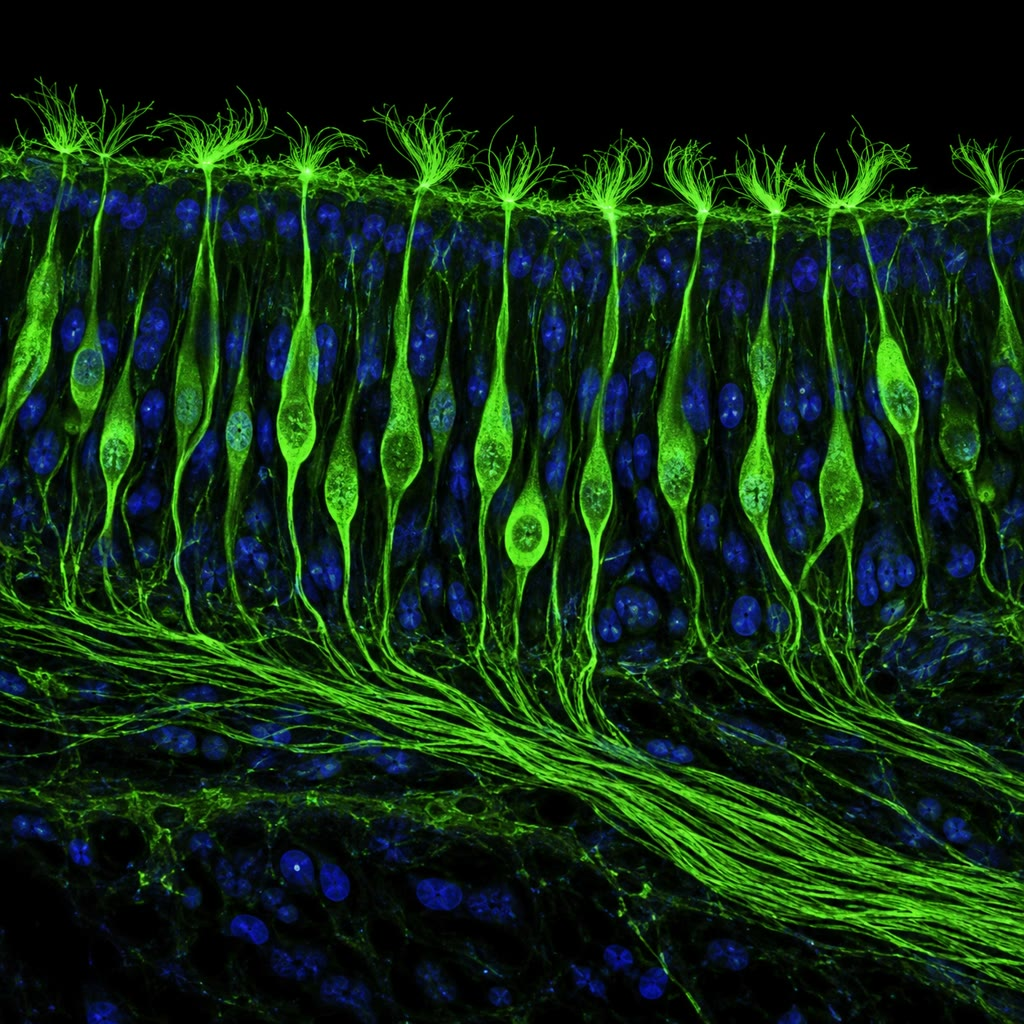
\includegraphics[width=0.40\linewidth]{images/book5/ai/b5-18-olfactory-epithelium.jpg}

{\small 嗅上皮：感觉神经元（绿色），其表面的树突带有\omterm{def:b3:cytoskeleton-motility:cilia}{纤毛}，
气味分子在此结合；轴突在其下方成束，
朝向嗅球走行。每个神经元表达
四百种受体基因中的一种。}
\end{omfigure}

\section{触觉、温度、痛觉与人类所缺乏的感觉}

\begin{definition}[体感觉]\label{def:b3:sensory-systems:somato}
\index{机械感受器}\index{Piezo 通道}\index{TRP 通道}\index{伤害感受器}\index{本体感觉}
皮肤中有多种\emph{机械感受器}，每种都是末端包裹在自身囊中的轴突：
默克尔细胞负责精细压力与质地（慢适应，小\omterm{def:b3:sensory-systems:principles}{感受野}），
迈斯纳小体负责轻触与滑动（快适应），
帕西尼小体位于皮肤深部，负责振动（极快适应，\omterm{def:b3:sensory-systems:principles}{感受野}很大），
鲁菲尼末梢感受
拉伸。多数此类感受器的换能器是\emph{Piezo2}，
一种巨大的离子通道，膜受牵张时开放，其上带有螺旋桨状的叶片；
若缺少它，触觉与身体位置觉均将丧失，
肺与膀胱中的同一通道则感知其充盈程度。
\emph{温度}由 TRP 家族的通道感受，
这些通道各自调谐于不同的温度范围：TRPV1 在高于
\qty{43}{\celsius} 的热刺激下开放，也可被辣椒素激活，这正是辣椒令人感到“辣”的原因；
TRPM8 则被冷刺激与薄荷醇激活，而\emph{疼痛}由游离神经末梢感受，
即\emph{伤害感受器}，它们对具破坏性的热刺激、压力
或化学物质（质子、ATP、缓激肽）作出反应，其阈值
因\omterm{def:b3:innate-immunity:inflammation}{炎症}而降低（见\cref{ch:b3:innate-immunity}）。
\emph{本体感觉}，即感知肢体所在位置的感觉，来自
肌梭与腱器官（见\cref{ch:b3:nervous-systems}），
以及关节囊中的 Piezo2。感受器的密度决定
敏锐度：两点相距 \qty{2}{mm} 时，指尖即可分辨，
背部则须相距 \qty{40}{mm} 方能分辨。
\end{definition}

\begin{method}[测量感觉]\label{met:b3:sensory-systems:psychophysics}
\index{心理物理学}\index{阈值}\index{两点辨别}
为刻画一条感觉通道：（1）求\emph{绝对阈值}，
即多次呈现强度分级的刺激，拟合被察觉的比例，
取被察觉比例为一半时的强度，
如赫克特所做的那样；（2）求\emph{差别阈值}，
在若干强度下测定，并检验韦伯定律；（3）测定\emph{空间敏锐度}，
用间距可变的两个刺激（皮肤上的两点测试，\omterm{def:b3:sensory-systems:retina}{视网膜}上的光栅）；
（4）测定\emph{时间敏锐度}，用闪烁或咔嗒声
（日间视觉下，约 \qty{60}{Hz} 的闪烁即可融合）；
（5）在动物身上，施加相同刺激时记录单根传入纤维的活动，
并使神经阈值与行为阈值相对应；
\omterm{met:b3:sensory-systems:psychophysics}{心理物理学}与生理学结果应当一致，若二者不一致，
其差异即为大脑所附加的部分。
\end{method}

\begin{remark}[其他动物，其他感觉]\label{rem:b3:sensory-systems:others}
本节所述的每种感觉，都有某种动物将其推进得更远，而且
还存在人类所缺乏的感觉。鲨鱼与鳐感知猎物心跳产生的
微伏级电场，借助充满凝胶的管道；电鱼则读取自身电场的畸变，
从而在黑暗中“看见”。蝮蛇用红外敏感的颊窝为
温热的猎物成像；蝙蝠与海豚进行回声定位，
测量自身叫声回声的时间，精确到几微秒，并
调节叫声频率以追踪飞蛾；蜜蜂能看见紫外线，并
感知天光的偏振，据此导航；迁徙的鸟类与
海龟则借助一种尚有争议的机制感知地磁场。
狗的鼻子所含受体神经元是人类的四十倍，
其脑的三分之一用于解读这些信号；猫头鹰能听见雪下的老鼠。
这些原理并未改变：换能器、\omterm{def:b3:sensory-systems:principles}{标记线路}、编码、
压缩、图谱，而多样性正是演化对这些原理所作的
改造。
\end{remark}

\section{练习}

\begin{exercise}[$\star$]\label{exo:b3:sensory-systems:1}
解释大脑如何判断一串脉冲来自眼睛还是耳朵，
已知这些脉冲完全相同。
\end{exercise}

\begin{exercise}[$\star$]\label{exo:b3:sensory-systems:2}
解释为何光会使光感受器超极化，
以及什么是暗电流。
\end{exercise}

\begin{exercise}[$\star$]\label{exo:b3:sensory-systems:3}
耳语为 \qty{20}{dB}，交谈为 \qty{60}{dB}，摇滚音乐会为
\qty{110}{dB}。计算三者各自的声强（单位 W/m$^{2}$），以及
最响与最轻之间的比值。
\end{exercise}

\begin{exercise}[$\star$]\label{exo:b3:sensory-systems:4}
列出五种\omterm{def:b3:sensory-systems:chemical}{味觉}模态及其受体类型，并解释
解释感冒为何会阻断食物的“味道”。
\end{exercise}

\begin{exercise}[$\star\star$]\label{exo:b3:sensory-systems:5}
体重的韦伯分数为 $0.02$。从 \qty{100}{g} 的体重起，
到 \qty{10}{kg} 为止，中间有多少个刚好可察觉的
差别台阶？用费希纳公式计算，并通过逐步数出
每步比值为 $1.02$ 的台阶数来检验。
\end{exercise}

\begin{exercise}[$\star\star$]\label{exo:b3:sensory-systems:6}
利用\cref{thm:b3:sensory-systems:hecht}，计算 $P_{\text{看见}}$，
对 $a = 2$、$6$ 和 $12$ 个被吸收的光子，阈值取 $n = 6$ 时的值。
闪光有一半时间被看见时 $a$ 为多少？若 \qty{10}{\%} 的光子
在角膜处被吸收，则闪光须发出多少个光子？
\end{exercise}

\begin{exercise}[$\star\star$]\label{exo:b3:sensory-systems:7}
中耳把来自 \qty{55}{mm^2} 面积的力集中到
\qty{3}{mm^2} 的面积上，杠杆比为 $1.3$。压强提高了多少倍，
以\omterm{def:b3:sensory-systems:cochlea}{分贝}计又提高多少？为什么中耳骨骼融合（耳硬化症）
患者的听觉会减弱数十\omterm{def:b3:sensory-systems:cochlea}{分贝}？
\end{exercise}

\begin{exercise}[$\star\star$]\label{exo:b3:sensory-systems:8}
解释为什么\omterm{def:b3:sensory-systems:cochlea}{毛细胞}的\omterm{def:b3:bacteriology:hgt}{转导}电流能在
微秒之内出现，而光感受器的\omterm{def:b3:bacteriology:hgt}{转导}电流要用
数十毫秒，以及两种感觉从这一设计中各获得了什么。
\end{exercise}

\begin{exercise}[$\star\star$]\label{exo:b3:sensory-systems:9}
小鼠有 \num{1100} 种受体类型，人类有 $400$ 种。若一种气味
大约激活 \qty{5}{\%} 的类型，则能形成恰好这一大小模式的
数目各为多少（取 $\binom{R}{k}$，$k = 0.05R$，
并用斯特林近似 $\ln\binom{R}{k} \approx R\,H(k/R)$，其中
$H(p) = -p\ln p - (1-p)\ln(1-p)$）？
\end{exercise}

\begin{exercise}[$\star\star\star$]\label{exo:b3:sensory-systems:10}
一个\omterm{def:b3:sensory-systems:retina}{视杆细胞}的\omterm{def:b3:sensory-systems:retina}{视紫红质}在黑暗中平均每
\qty{40}{s} 自发异构化一次。在 $500$ 个\omterm{def:b3:sensory-systems:retina}{视杆细胞}组成的区域中，
观察 \qty{0.1}{s} 的时间窗，平均自发事件数是多少，以及
偶然发生六次或更多次的概率是多少？试说明大脑为何将
阈值设在六次左右，而不是一次。
\end{exercise}

\begin{exercise}[$\star\star\star$]\label{exo:b3:sensory-systems:11}
听神经的放电锁定于声音的相位，直到
\qty{4}{kHz}，抖动约为 \qty{20}{\micro s}。声音以 \qty{340}{m/s} 传播，两耳相距 \qty{20}{cm}。
最大耳间延迟是多少？
在中线附近，\qty{10}{\micro s} 的辨别能给出多大的角\omterm{def:b3:structural-biology:methods}{分辨率}？
以及为什么高于 \qty{4}{kHz} 时起作用的是位置编码，
而不是时序？
\end{exercise}

\begin{exercise}[$\star\star\star$]\label{exo:b3:sensory-systems:12}
\omterm{def:b3:sensory-systems:principles}{侧向抑制}使紧邻暗区的一块均匀灰场
在边界处显得更亮。建立一排感受器的模型，每个感受器由
自身光照 $I_{i}$ 激发，并受每个邻居光照的 $w$ 比例抑制，
即 $r_{i} = I_{i} - w(I_{i-1} + I_{i+1})$，并计算从
$I = 1$ 到 $I = 2$ 的阶跃处的响应，取 $w = 0.2$。\omterm{def:b3:sensory-systems:retina}{视网膜}由此获得了什么，
又失去了什么？
\end{exercise}

\section{问题：远处所见的烛光}

\begin{problem}[{周末问题——远处眼睛所计数的烛光光子，
由泊松统计算出闪光的探测情况，以及视杆细胞的放大器，
一场音乐会的分贝数换算为鼓膜运动和毛细胞电流，
以及鼻子编码的枚举，最后归结于烛光可被看见的距离、
鼓膜处的压强，以及鼻子能形成的
模式数}]
\label{pb:b3:sensory-systems:1}
数据：蜡烛发出约 \qty{0.01}{W} 的可见光，
波长为 \qty{550}{nm}（光子能量 $3.6\times 10^{-19}$ J）。暗适应后的
瞳孔直径为 \qty{7}{mm}；进入眼睛的光子中有 \qty{10}{\%}
被\omterm{def:b3:sensory-systems:retina}{视紫红质}吸收；眼睛在 \qty{0.1}{s} 内积分；
阈值为 $6$ 个被吸收的光子。每个被吸收的光子关闭 $200$
个通道，使暗电流减少 \qty{1}{pA}，持续 \qty{0.2}{s}；
\omterm{def:b3:sensory-systems:retina}{视杆细胞}的暗电流为 \qty{30}{pA}。声音：$I_{0} =
\qty{1e-12}{W/m^2}$；鼓膜面积为 \qty{55}{mm^2}；毛束
高度为 \qty{5}{\micro m}，阈值处偏转 \qty{0.3}{nm}。
嗅觉：$R = 400$ 个受体；一个\omterm{def:b3:sensory-systems:cochlea}{毛细胞}的\omterm{def:b3:bacteriology:hgt}{转导}电流在
饱和时为 \qty{100}{pA}。

\medskip
\noindent\textbf{第一部分——光子。}
\begin{enumerate}
  \item 蜡烛每秒发出多少个光子？
  \item 在距离 $d$ 处，光子均匀分布于面积为
        $4\pi d^{2}$ 的球面上。每秒有多少光子进入瞳孔，
        在 \qty{1}{km} 处？\qty{10}{km} 处又是多少？
  \item 在每个距离处，一个积分时间窗内被吸收的
        光子有多少个？烛光能被看见吗（阈值为 $6$）？
  \item 求使一个时间窗内被吸收光子的平均数等于 $6$ 的
        距离。用泊松统计，此距离处有多大比例的时间窗
        超过阈值？
  \item 在第 4 题的距离处，任一给定的 \qty{0.1}{s} 时间窗
        内完全不含光子的概率是多少？为什么一颗
        暗淡的恒星看起来会闪烁？
  \item 在满月照耀下，同样的\omterm{def:b3:sensory-systems:retina}{视杆细胞}每个时间窗从天空中
        吸收 $10^{4}$ 个光子。试说明为何在 \qty{10}{km} 处的烛光
        此时不可见，尽管它送来的光子数相同。
\end{enumerate}

\medskip
\noindent\textbf{第二部分——\omterm{def:b3:sensory-systems:retina}{视杆细胞}的放大器。}
\begin{enumerate}[resume]
  \item 一个光子关闭 $200$ 个通道，使电流减小
        \qty{1}{pA}。单个通道携带多大电流，每秒
        通过的阳离子数是多少（$e = \qty{1.6e-19}{C}$）？
  \item 一个光子去除了暗电流的多大比例？要使\omterm{def:b3:sensory-systems:retina}{视杆细胞}
        同时吸收多少个光子才能使其完全关闭
        （饱和）？
  \item 响应持续 \qty{0.2}{s}。一个光子使多少个阳离子
        无法进入细胞？每个
        光子的电荷增益是多少？
  \item 白天每秒有 $10^{5}$ 个光子到达一个\omterm{def:b3:sensory-systems:retina}{视杆细胞}。
        它会发生什么？为什么较不易适应、也较不易饱和的\omterm{def:b3:sensory-systems:retina}{视锥细胞}
        是白天的感受器？
  \item \omterm{def:b3:sensory-systems:retina}{视锥细胞}约需 $100$ 个光子才能发出信号。从灵敏度与速度的
        权衡角度，说明为何\omterm{def:b3:sensory-systems:retina}{视锥细胞}的响应
        在 \qty{20}{ms} 内，而\omterm{def:b3:sensory-systems:retina}{视杆细胞}在 \qty{200}{ms} 内。
  \item \omterm{def:b3:sensory-systems:retina}{视紫红质}平均每 \qty{40}{s} 自发异构化一次。对
        一只眼睛中的 $10^{8}$ 个\omterm{def:b3:sensory-systems:retina}{视杆细胞}，\omterm{def:b3:sensory-systems:retina}{视网膜}每秒
        产生多少个假光子？为什么这不会使暗处的
        眼睛被噪声致盲？（请考虑阈值与
        \omterm{def:b3:sensory-systems:principles}{感受野}。）
\end{enumerate}

\medskip
\noindent\textbf{第三部分——\omterm{def:b3:sensory-systems:cochlea}{分贝}。}
\begin{enumerate}[resume]
  \item 一场 \qty{110}{dB} 的音乐会，求其强度
        （以 W/m$^{2}$ 计）以及落在一只鼓膜上的功率。
  \item 两小时的音乐会中，鼓膜接收多少声能？
        请与一滴下落雨滴的能量作比较，
        雨滴能量为 \qty{1e-4}{J}。
  \item 听阈为 \qty{0}{dB} 时鼓膜上的功率，
        以及每 \qty{10}{ms} 内的能量 ---
        与一个可见光光子的能量作比较。
  \item 听阈处，高 \qty{5}{\micro m} 的听毛束偏转 \qty{0.3}{nm}，
        其偏转角为多少度？并将该偏转量
        与一个氢原子的直径作比较，氢原子直径为
        \qty{0.1}{nm}。
  \item 在超过 \qty{85}{dB} 的环境中长时间暴露会\omterm{def:b3:dna-repair:lesions}{损伤}\omterm{def:b3:sensory-systems:cochlea}{毛细胞}，
        而哺乳动物的\omterm{def:b3:sensory-systems:cochlea}{毛细胞}不能再生。在 \qty{110}{dB} 下
        持续两小时所接收的能量，相当于在 \qty{85}{dB} 下
        持续多少小时？
  \item 听力范围为 \qty{120}{dB}。若强度的韦伯分数约为
        $0.25$（即一\omterm{def:b3:sensory-systems:cochlea}{分贝}），可觉察的响度差别
        共有多少级？
\end{enumerate}

\medskip
\noindent\textbf{第四部分——嗅觉编码。}
\begin{enumerate}[resume]
  \item 若 $400$ 个受体各自只有“开”或“关”两种状态，共有多少种模式？
        请将结果写成十的幂次。
  \item 若一种气味通常激活 $20$ 个受体，则
        这样互不相同的模式有多少种（$\binom{400}{20}$，
        可用斯特林公式或取对数计算）？
  \item 两种气味物质共享 $15$ 个受体，而各自的受体总数均为 $20$ 个。
        试在编码中提出一种衡量二者距离的度量，并解释
        它们为何闻起来相似。
  \item 人类约能分辨一万亿种气味。这占第 20 题中模式数的
        多大比例？又是什么限制了可分辨的数目，
        使其远低于编码容量？
  \item 一只拥有 \num{1100} 个受体的小鼠，其 $20$ 个受体组合的模式
        比人类多出多少种？请以十的幂次表示。
  \item 一次突变删除了一个受体基因。试预测这一突变对总体嗅觉能力的影响，
        以及对与该受体强烈结合的某一种气味物质的感知的影响
        （特异性嗅觉缺失）。
  \item 综合：蜡烛被看见的距离
        （第~4 题）、听阈时鼓膜上的声能
        （每 \qty{10}{ms} 内，第~15 题），以及人类鼻子
        能形成的二十受体模式数（第~20 题）。
\end{enumerate}
\end{problem}
